\chapter{Related Works}

Your related works, and your purpose and contribution which.
\section{Tasya Wiendhyra/1164086}
\subsection{binary classification dilengkapi ilustrasi gambar}
\begin{enumerate}
\item Binary classification yaitu berupa kelas positif dan kelas negatif. Klasifikasi biner adalah dikotomisasi yang diterapkan untuk tujuan praktis, dan dalam banyak masalah klasifikasi biner praktis, kedua kelompok tidak simetris - daripada akurasi keseluruhan, proporsi relatif dari berbagai jenis kesalahan yang menarik. Misalnya, dalam pengujian medis, false positive (mendeteksi penyakit ketika tidak ada) dianggap berbeda dari false negative (tidak mendeteksi penyakit ketika hadir).
\begin{figure}[ht]
\centering
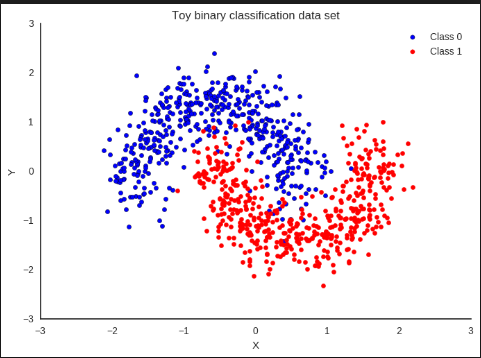
\includegraphics[scale=0.5]{figures/wiendh1.png}
\caption{Binary Classification}
\label{contoh}
\end{figure}
\end{enumerate}

\subsection{supervised learning dan unsupervised learning dan clustering dengan ilustrasi gambar}
\begin{enumerate}
\item Supervised learning adalah tugas pembelajaran mesin untuk mempelajari suatu fungsi yang memetakan input ke output berdasarkan contoh pasangan input-output. Ini menyimpulkan fungsi dari data pelatihan berlabel yang terdiri dari serangkaian contoh pelatihan. Dalam pembelajaran yang diawasi, setiap contoh adalah pasangan yang terdiri dari objek input (biasanya vektor) dan nilai output yang diinginkan (juga disebut sinyal pengawas). Algoritma pembelajaran yang diawasi menganalisis data pelatihan dan menghasilkan fungsi yang disimpulkan, yang dapat digunakan untuk memetakan contoh-contoh baru. Skenario optimal akan memungkinkan algoritma menentukan label kelas dengan benar untuk instance yang tidak terlihat. Ini membutuhkan algoritma pembelajaran untuk menggeneralisasi dari data pelatihan untuk situasi yang tidak terlihat dengan cara yang "masuk akal" (lihat bias induktif). Tugas paralel dalam psikologi manusia dan hewan sering disebut sebagai pembelajaran konsep. Contoh dibawah yaitu Supervised Learning dengan SVC.
\begin{figure}[ht]
\centering
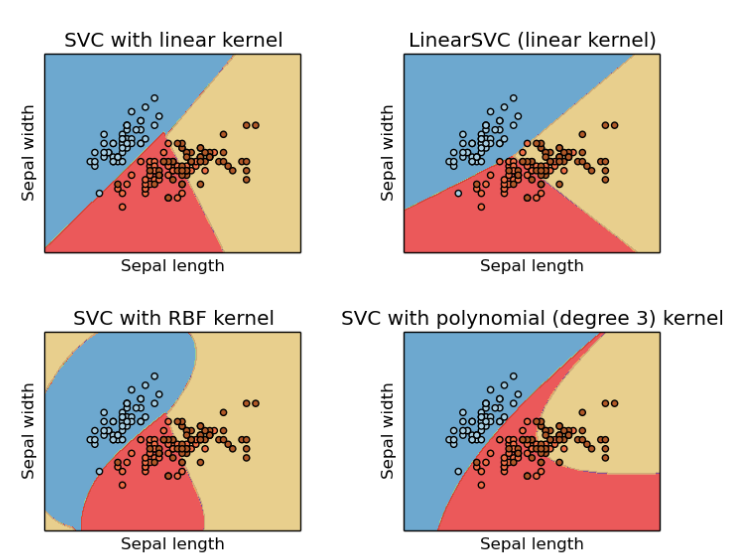
\includegraphics[scale=0.5]{figures/wiendh2.png}
\caption{Supervised Learning}
\label{contoh}
\end{figure}
\item Unsupervised learning adalah istilah yang digunakan untuk pembelajaran bahasa Ibrani, yang terkait dengan pembelajaran tanpa guru, juga dikenal sebagai organisasi mandiri dan metode pemodelan kepadatan probabilitas input. Analisis cluster sebagai cabang pembelajaran mesin yang mengelompokkan data yang belum diberi label, diklasifikasikan atau dikategorikan. Alih-alih menanggapi umpan balik, analisis klaster mengidentifikasi kesamaan dalam data dan bereaksi berdasarkan ada tidaknya kesamaan di setiap potongan data baru. BErikut merupakan contoh Unsupervised Learning dengan Gaussian mixture models.
\begin{figure}[ht]
\centering
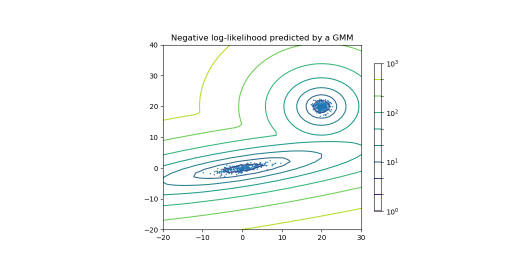
\includegraphics[scale=0.5]{figures/wiendh3.png}
\caption{Unsupervised Learning}
\label{contoh}
\end{figure}
\item Cluster analysis or clustering adalah tugas pengelompokan sekumpulan objek sedemikian rupa sehingga objek dalam kelompok yang sama (disebut klaster) lebih mirip (dalam beberapa hal) satu sama lain daripada pada kelompok lain (kluster). Ini adalah tugas utama penambangan data eksplorasi, dan teknik umum untuk analisis data statistik, yang digunakan di banyak bidang, termasuk pembelajaran mesin, pengenalan pola, analisis gambar, pengambilan informasi, bioinformatika, kompresi data, dan grafik komputer. Analisis Cluster sendiri bukan merupakan salah satu algoritma spesifik, tetapi tugas umum yang harus dipecahkan. Ini dapat dicapai dengan berbagai algoritma yang berbeda secara signifikan dalam pemahaman mereka tentang apa yang merupakan sebuah cluster dan bagaimana cara menemukannya secara efisien. Gagasan populer mengenai cluster termasuk kelompok dengan jarak kecil antara anggota cluster, area padat ruang data, interval atau distribusi statistik tertentu. Clustering karena itu dapat dirumuskan sebagai masalah optimasi multi-objektif. Algoritma pengelompokan dan pengaturan parameter yang sesuai (termasuk parameter seperti fungsi jarak yang akan digunakan, ambang kepadatan atau jumlah cluster yang diharapkan) tergantung pada set data individual dan penggunaan hasil yang dimaksudkan. Analisis kluster bukan merupakan tugas otomatis, tetapi proses berulang penemuan pengetahuan atau optimasi multi-objektif interaktif yang melibatkan percobaan dan kegagalan. Seringkali diperlukan untuk memodifikasi praproses data dan parameter model hingga hasilnya mencapai properti yang diinginkan.
\begin{figure}[ht]
\centering
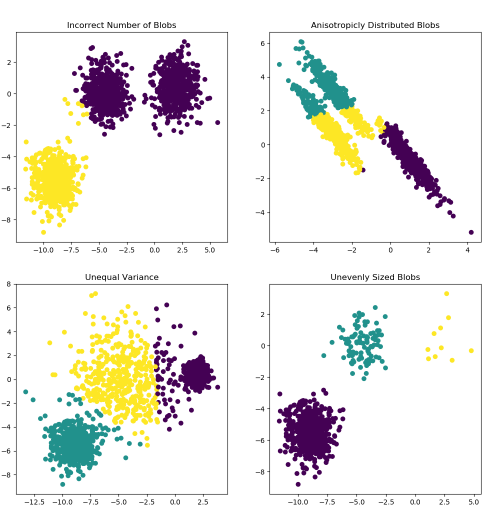
\includegraphics[scale=0.5]{figures/wiendh4.png}
\caption{Cluster}
\label{contoh}
\end{figure}
\end{enumerate}

\subsection{evaluasi dan akurasi dari buku dan disertai ilustrasi contoh
dengan gambar}
\begin{enumerate}
\item Evaluasi adalah tentang  bagaimana kita dapat mengevaluasi seberapa baik model bekerja dengan mengukur akurasinya. Dan akurasi akan didefinisikan sebagai persentase kasus yang diklasifikasikan dengan benar. Kita dapat menganalisis kesalahan yang dibuat oleh model, atau tingkat kebingungannya, menggunakan matriks kebingungan. Matriks kebingungan mengacu pada kebingungan dalam model, tetapi matriks kebingungan ini bisa menjadi sedikit sulit untuk dipahami ketika mereka menjadi sangat besar.
\begin{figure}[ht]
\centering
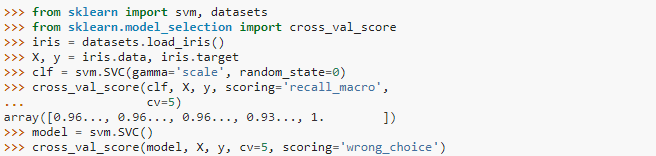
\includegraphics[scale=0.5]{figures/wiendh9.png}
\caption{ Evaluasi dan Akurasi}
\label{contoh}
\end{figure}
\end{enumerate}

\subsection{ bagaimana cara membuat dan membaca confusion matrix, buat confusion matrix }
\begin{enumerate}
\item Cara membuat dan membaca confusion matrix :
\begin{itemize}
\item 1)	Tentukan pokok permasalahan dan atributanya, misal gaji dan listik.
\item 2)	Buat pohon keputusan
\item 3)	Lalu data testingnya
\item 4)	Lalu mencari nilai a, b, c, dan d. Semisal a = 5, b = 1, c = 1, dan d = 3.
\item 5)	Selanjutnya mencari nilai recall, precision, accuracy, serta dan error rate.
\end{itemize}
\item Berikut adalah contoh dari confusion matrix :
\begin{itemize}
\item Recall =3/(1+3) = 0,75
\item Precision = 3/(1+3) = 0,75
\item Accuracy =(5+3)/(5+1+1+3) = 0,8
\item Error Rate =(1+1)/(5+1+1+3) = 0,2
\end{itemize}
\end{enumerate}

\subsection{bagaimana K-fold cross validation bekerja dengan gambar ilustrasi}
\begin{enumerate}
\item Cara kerja K-fold cross validation :
\begin{itemize}
\item 1)	Total instance dibagi menjadi N bagian.
\item 2)	Fold yang pertama adalah bagian pertama menjadi data uji (testing data) dan sisanya menjadi training data.
\item 3)	Lalu hitung akurasi berdasarkan porsi data tersebut dengan menggunakan persamaan.
\item 4)	Fold yang ke dua adalah bagian ke dua menjadi data uji (testing data) dan sisanya training data. 
\item 5)	Kemudian hitung akurasi berdasarkan porsi data tersebut.
\item 6)	Dan seterusnya hingga habis mencapai fold ke-K.
\item 7)	Terakhir hitung rata-rata akurasi K buah.
\end{itemize}
\begin{figure}[ht]
\centering
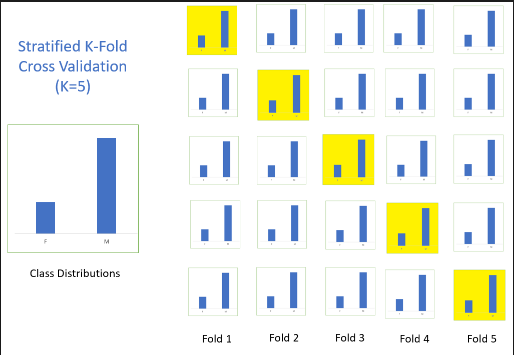
\includegraphics[scale=0.5]{figures/wiendh5.png}
\caption{K-fold cross validation }
\label{contoh}
\end{figure}
\end{enumerate}

\subsection{decision tree dengan gambar ilustrasi}
\begin{enumerate}
\item Decision Tree dalah metode pembelajaran yang diawasi non-parametrik yang digunakan untuk klasifikasi dan regresi. Tujuannya adalah untuk membuat model yang memprediksi nilai variabel target dengan mempelajari aturan keputusan sederhana yang disimpulkan dari fitur data.\\
Misalnya, dalam contoh di bawah ini, decision tree belajar dari data untuk memperkirakan kurva sinus dengan seperangkat aturan keputusan if-then-else. Semakin dalam pohon, semakin rumit aturan keputusan dan semakin bugar modelnya.
\begin{figure}[ht]
\centering
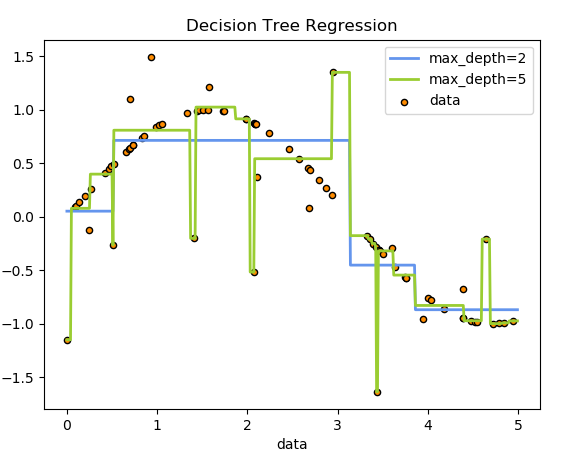
\includegraphics[scale=0.5]{figures/wiendh6.png}
\caption{Decision Tree}
\label{contoh}
\end{figure}
\end{enumerate}

\subsection{Information Gain dan entropi dengan gambar ilustrasi}
\begin{enumerate}
\item Information gain didasarkan pada penurunan entropi setelah dataset dibagi pada atribut. Membangun decision tree adalah semua tentang menemukan atribut yang mengembalikan perolehan informasi tertinggi (mis., Cabang yang paling homogen).
\begin{figure}[ht]
\centering
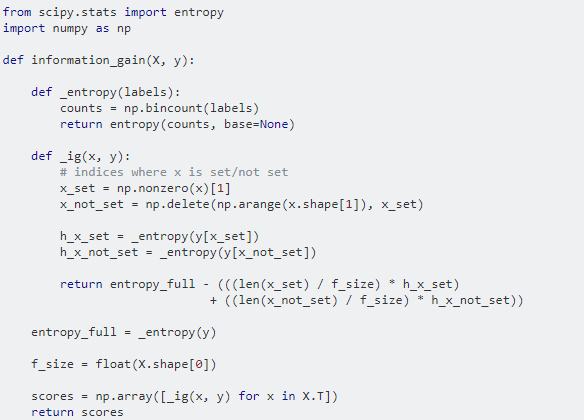
\includegraphics[scale=0.5]{figures/wiendh7.png}
\caption{Information gain}
\label{contoh}
\end{figure}
\item Entropi adalah ukuran keacakan dalam informasi yang sedang diproses. Semakin tinggi entropi, semakin sulit untuk menarik kesimpulan dari informasi itu. Membalik koin adalah contoh tindakan yang memberikan informasi yang acak. Untuk koin yang tidak memiliki afinitas untuk kepala atau ekor, hasil dari sejumlah lemparan sulit diprediksi. Mengapa? Karena tidak ada hubungan antara membalik dan hasilnya. Inilah inti dari entropi.
\begin{figure}[ht]
\centering
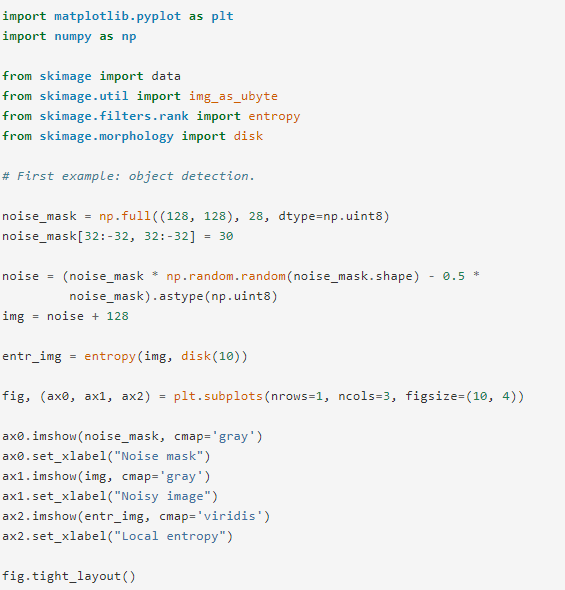
\includegraphics[scale=0.5]{figures/wiendh8.png}
\caption{Entropi}
\label{contoh}
\end{figure}
\end{enumerate}

\section{scikit-learn}
HARI KEDUA TASYA WIENDHYRA 1164086

\begin{enumerate}

\item
\begin{verbatim}
	# load dataset (student mat pakenya)
	import pandas as pd
	durian = pd.read_csv('student-mat.csv', sep=';')
	len(d)
\end{verbatim}

\par
Codingan diatas digunakan untuk mengimport atau memanggil module pandas sebagai pd. Kemudian mendefinisikan variabel "durian" yang akan memanggil dataset yang didapatkan dari data csv. Jika skrip dijalankan di Spyder, hasilnya seperti berikut 
\begin{figure}[ht]
\centering
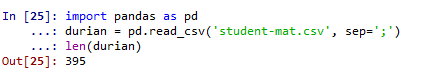
\includegraphics[scale=0.5]{figures/spyder1.png}
\caption{Loading Dataset}
\label{Spyder}
\end{figure}
\item
\begin{verbatim}
	# generate binary label (pass/fail) based on G1+G2+G3 
	# (test grades, each 0-20 pts); threshold for passing is sum>=30
	durian['pass'] = durian.apply(lambda row: 1 if (row['G1']+row['G2']+row['G3']) 
											>= 35 else 0, axis=1)
	durian = durian.drop(['G1', 'G2', 'G3'], axis=1)
	durian.head()
\end{verbatim}

\par
ada bagian ini mendeklarasikan pass/fail nya data berdasarkan G1+G2+G3. Dengan ketentuan nilai pass nya yaitu sama dengan 30.
kemudian pada variabel durian dideklarasikan  jika baris dengan G1+G2+G3 ditambahkan, dan hasilnya sama dengan 35 maka axisnya 1. ketika dijalankan hasilnya seperti berikut
\begin{figure}[ht]
\centering
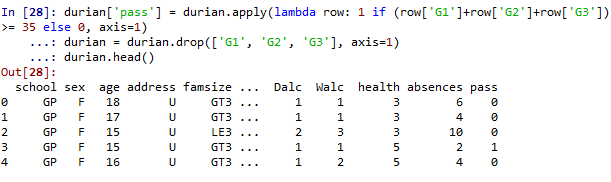
\includegraphics[scale=0.5]{figures/spyder2.png}
\caption{Generate Binary Label}
\label{Spyder}
\end{figure}
\item
\begin{verbatim}
	# use one-hot encoding on categorical columns
	durian = pd.get_dummies(durian, columns=['sex', 'school', 'address', 
									'famsize', 
									'Pstatus', 'Mjob', 'Fjob', 
	                               'reason', 'guardian', 'schoolsup', 
								   'famsup', 'paid', 'activities',
	                               'nursery', 'higher', 'internet', 
									'romantic'])
	durian.head()
\end{verbatim}
\par
One-hot encoding adalah proses di mana variabel kategorikal dikonversi menjadi bentuk yang dapat disediakan untuk algoritma ML untuk melakukan pekerjaan yang lebih baik dalam prediksi. Karena saya memuat data menggunakan panda, disini menggunakan fungsi panda pdgetdummies untuk jenis kelamin , sekolah, alamat dll. Metode head ini digunakan untuk mengembalikan baris n atas 5 secara default dari frame atau seri data. hasilnya seperti berikut 
\begin{figure}[ht]
\centering
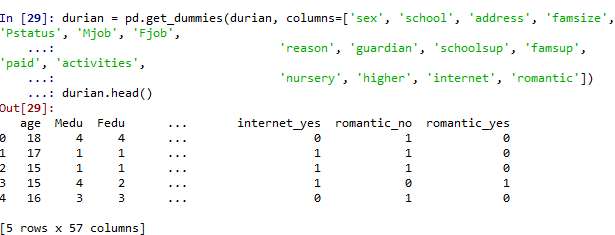
\includegraphics[scale=0.5]{figures/spyder3.png}
\caption{One-hot Encoding}
\label{Spyder}
\end{figure}
\item
\begin{verbatim}
	# shuffle rows
	durian = durian.sample(frac=1)
	# split training and testing data
	durian_train = d[:500]
	durian_test = d[500:]

	durian_train_att = durian_train.drop(['pass'], axis=1)
	durian_train_pass = durian_train['pass']

	durian_test_att = durian_test.drop(['pass'], axis=1)
	durian_test_pass = durian_test['pass']

	durian_att = durian.drop(['pass'], axis=1)
	durian_pass = d['pass']

	# number of passing students in whole dataset:
	import numpy as np
	print("Passing: %d out of %d (%.2f%%)" % (np.sum(d_pass), len(d_pass), 
	       100*float(np.sum(d_pass)) / len(d_pass)))
\end{verbatim}

\par
Sammple digunakan untuk mengembalikan sampel acak item dari objek. Pada bagian tersebut, terdapat train dan test yaing digunakan untuk untuk membagi train, test dan kemudian membagi lagi train ke validasi dan test.\\
Kemudia akan mengimport module numpy sebagai np yang akan digunakan untuk mengembalikan nilai passing dari pelajar dari keseluruhan dataset dengan cara print.
\begin{figure}[ht]
\centering
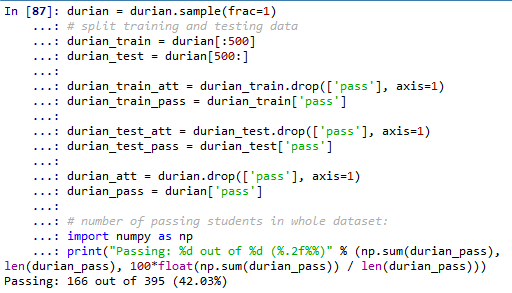
\includegraphics[scale=0.5]{figures/spyder4.png}
\caption{Shuffle Rows}
\label{Spyder}
\end{figure}
\item 
\begin{verbatim}
	# fit a decision tree
	from sklearn import tree
	mangga = tree.DecisionTreeClassifier(criterion="entropy", max_depth=5)
	mangga = mangga.fit(durian_train_att, durian_train_pass)
\end{verbatim}

\par
Dari librari scikitlearn import modul tree. Kemudian definisikan variabel Mangga dengan menggunakan DecisionClassifier. KEmudian pada variabel mangga terdapat Criterion yaitu suatu fungsi untuk mengukur kualitas split, setelah itu agar DecisionTreeClassifier dapat dijalankan gunakan perintah fit. hasilnya seperti dibawah
\begin{figure}[ht]
\centering
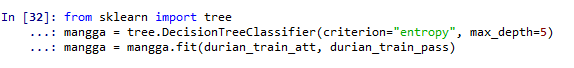
\includegraphics[scale=0.5]{figures/spyder5.png}
\caption{Fit Decision Tree}
\label{Spyder}
\end{figure}
\item
\begin{verbatim}
	# visualize tree
	import graphviz
	dot_data = tree.export_graphviz(mangga, out_file=None, label="all", 
									impurity=False, proportion=True,
	                                feature_names=list(durian_train_att), 
									class_names=["fail", "pass"], 
	                                filled=True, rounded=True)
	graph = graphviz.Source(dot_data)
	graph
\end{verbatim}

\par
Graphviz adalah perangkat lunak visualisasi grafik open source. Visualisasi grafik adalah cara mewakili informasi struktural sebagai diagram grafik dan jaringan abstrak. TREEEXPORTGRAPHVIZ merupakan fungsi yang menghasilkan representasi Graphviz dari decision tree, yang kemudian ditulis ke outfile. Sehingga akan muncul gambardiagram  grafik bercabang.
\begin{figure}[ht]
\centering
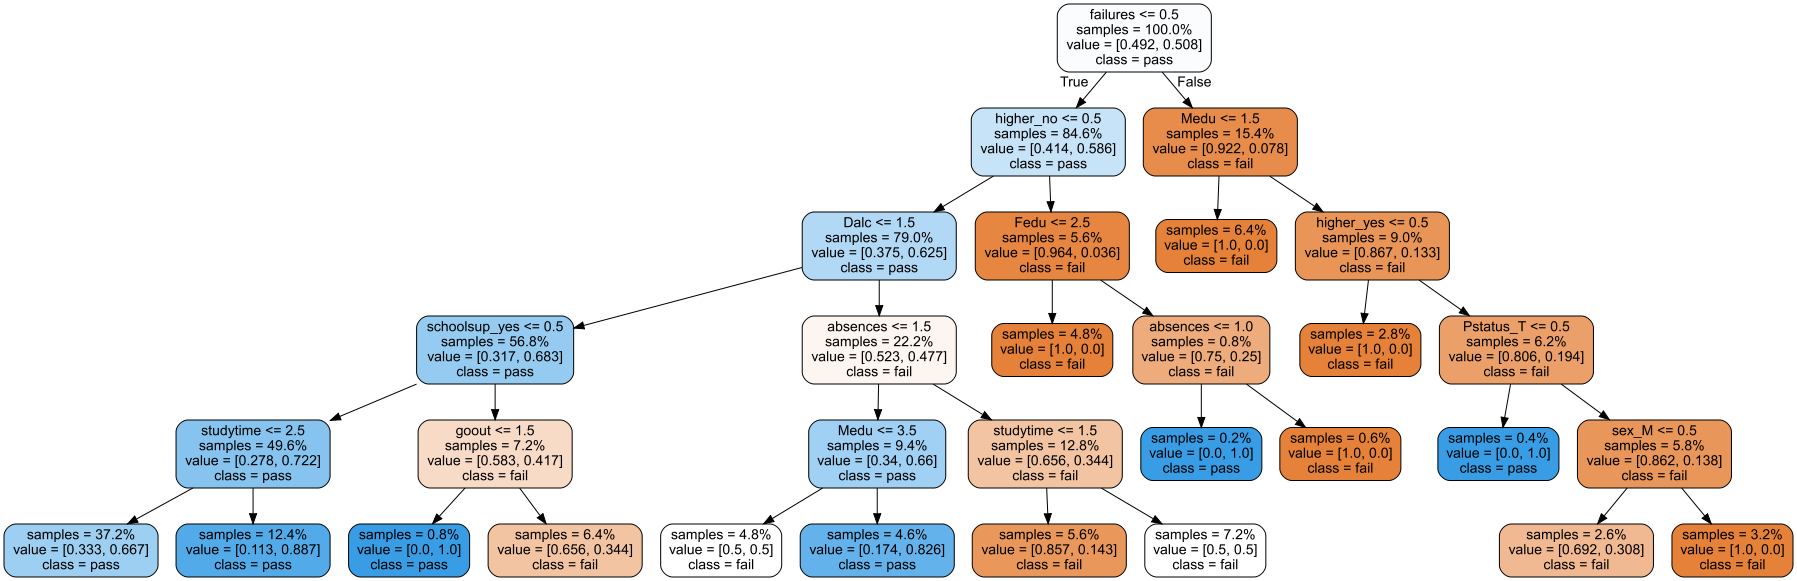
\includegraphics[scale=0.5]{figures/spyder6.png}
\caption{Fit Decision Tree}
\label{Spyder}
\end{figure}
\item
\begin{verbatim}
	# save tree
	tree.export_graphviz(mangga, out_file="student-performance.dot", 
						 label="all", impurity=False, 
						 proportion=True,
	                     feature_names=list(durian_train_att), 
	                     class_names=["fail", "pass"], 
	                     filled=True, rounded=True)
\end{verbatim}

\par
TREEEXPORTGRAPHVIZ merupakan fungsi yang menghasilkan representasi Graphviz dari decision tree, yang kemudian ditulis ke outfile.Disini akan menyimpan classifiernya, akan meng ekspor file student performance jika salah akan mengembalikan nilai fail.
\begin{figure}[ht]
\centering
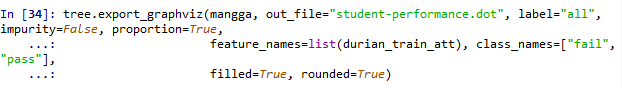
\includegraphics[scale=0.5]{figures/spyder7.png}
\caption{Fit Decision Tree}
\label{Spyder}
\end{figure}
\item
\begin{verbatim}
	mangga.score(durian_test_att, durian_test_pass)
\end{verbatim}

\par
Score juga disebut prediksi, dan merupakan proses menghasilkan nilai berdasarkan model pembelajaran mesin yang terlatih, diberi beberapa data input baru. Nilai atau skor yang dibuat dapat mewakili prediksi nilai masa depan, tetapi mereka juga mungkin mewakili kategori atau hasil yang mungkin. Jadi disini Mangga akan memprediksi nilai dari durian test att dan test pass. Hasilnya seperti dibawah ini
\begin{figure}[ht]
\centering
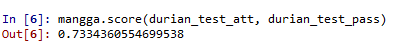
\includegraphics[scale=0.5]{figures/spyder8.png}
\caption{Score}
\label{Spyder}
\end{figure}
\item
\begin{verbatim}
	from sklearn.model_selection import cross_val_score
	nangka = cross_val_score(mangga, durian_att, durian_pass, cv=5)
	# show average score and +/- two standard deviations away 
	#(covering 95% of scores)
	print("Accuracy: %0.2f (+/- %0.2f)" % (nangka.mean(), nangka.std() * 2))
\end{verbatim}

\par
Skrip ini akan mengevaluasi score dengan validasi silang. Dimana variabel nangka berisikan crossvalscore yang merupakan fungsi pembantu pada estimator dan dataset. Kemudian akan menampilkan score rata rata dan kurang lebih dua standar deviasi yang mencakup 95 persen score. dengan menggunakan perintah print hasil yang didapatkan sebagai berikut
\begin{figure}[ht]
\centering
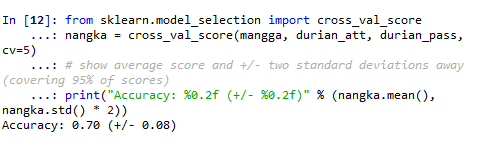
\includegraphics[scale=0.5]{figures/spyder9.png}
\caption{Cross Val Score}
\label{Spyder}
\end{figure}
\item 
\begin{verbatim}
	for max_depth in range(1, 20):
	    mangga = tree.DecisionTreeClassifier(criterion="entropy", 
			max_depth=max_depth)
	    nangka = cross_val_score(mangga, durian_att, durian_pass, cv=5)
	    print("Max depth: %d, Accuracy: %0.2f (+/- %0.2f)" % 
				(max_depth, nangka.mean(), nangka.std() * 2)
			 )
\end{verbatim}

\par
Pada skrip ini menunjukkan seberapa dalam tree itu. Semakin dalam tree, semakin banyak perpecahan yang dimilikinya dan menangkap lebih banyak informasi tentang data. variabel mangga akan mendefinisikan tree nya yang kemudian variabel nangka akan mengevaluasi score dengan validasi silang. disini mendefinisikan decision tree dengan kedalaman mulai dari 1 hingga 20 dan merencanakan pelatihan dan menguji skor auc. Jika di run hasilnya seperti berikut
\begin{figure}[ht]
\centering
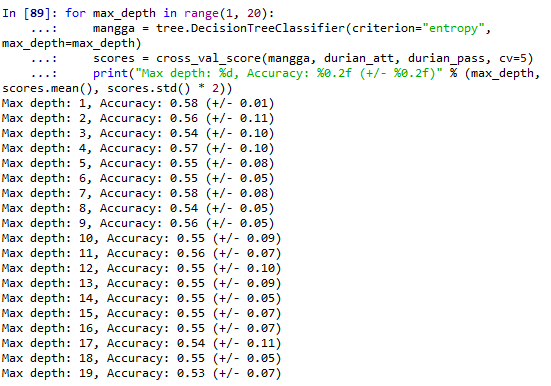
\includegraphics[scale=0.5]{figures/spyder10.png}
\caption{Max Depth}
\label{Spyder}
\end{figure}
\item
\begin{verbatim}
	depth_acc = np.empty((19,3), float)
	i = 0
	for max_depth in range(1, 20):
	    mangga = tree.DecisionTreeClassifier(criterion="entropy", 
			max_depth=max_depth)
	    nangka = cross_val_score(t, d_att, d_pass, cv=5)
	    depth_acc[i,0] = max_depth
	    depth_acc[i,1] = nangka.mean()
	    depth_acc[i,2] = nangka.std() * 2
	    i += 1

	depth_acc
\end{verbatim}

\par
Depth acc akan membuat array kosong dengan mengembalikan array baru dengan bentuk dan tipe yang diberikan, tanpa menginisialisasi entri. Dengan 19 sebagai bentuk array kosong, 3 sebagai output data-type dan float urutan kolom-utama (gaya Fortran) dalam memori. variabel mangga yang akan melakukan split score dan nangka akan mengvalidasi score secara silang. dan pada akhirnya nangka std yaitu menghitung standar deviasi dari data yang diberikan (elemen array) di sepanjang sumbu yang ditentukan (jika ada), hasilnya sebagai berikut
\begin{figure}[ht]
\centering
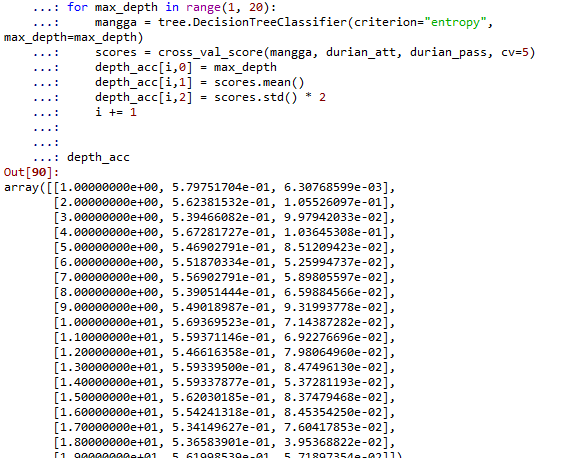
\includegraphics[scale=0.5]{figures/spyder11.png}
\caption{Depth in Range}
\label{Spyder}
\end{figure}
\item 
\begin{verbatim}
	import matplotlib.pyplot as plt
	fig, ax = plt.subplots()
	ax.errorbar(depth_acc[:,0], depth_acc[:,1], yerr=depth_acc[:,2])
	plt.show()
\end{verbatim}

\par
Mengimpor librari dari matplotlib yaitu pylot sebagai plt\\
fig dan ax menggunakan subplots untuk membuat gambar dan satu set subplot.\\
axerrorbar akan membuat error bar
kemudian grafik akan ditampilkan menggunakan show. Grafiknya seperti berikut
\\
\\
\\
\begin{figure}[ht]
\centering
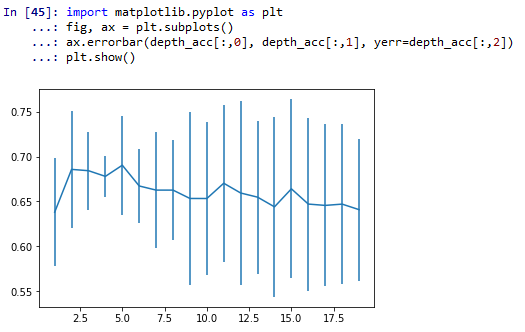
\includegraphics[scale=0.5]{figures/spyder12.png}
\caption{Matplotlib}
\label{Spyder}
\end{figure}
\end{enumerate}


\section{Penanganan Error}
HARI KEDUA TASYA WIENDHYRA 1164086
\subsection{Error Graphviz}
\begin{enumerate}
	\item
Berikut ini merupakan eror yang didapatkan saat menjalankan graphviz pada Spyder
\begin{figure}[ht]
\centering
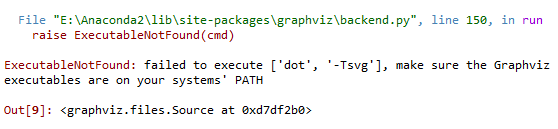
\includegraphics[scale=0.5]{figures/erorspyder1.png}
\caption{Error Graphviz}
\label{Error}
\end{figure}
	\item
Pada gambar diatas kode erornya adalah ExecutableNotFound failed to execute dot Tsvg. Eror ini terjadi karena tidak terdaftarnya environment variable dari Graphviz pada PATH di PC.
	\item
Solusi yang bisa dilakukan untuk mengatasi eror tersebut adalah sebagai berikut : \\
\begin{itemize}
\item
Buka Folder dimana Anaconda2 terinstall. Disini Anacondanya terinstal di folder E
\item
Kemudian, pada Anaconda2 buka Library/Bin/graphviz
\begin{figure}[ht]
\centering
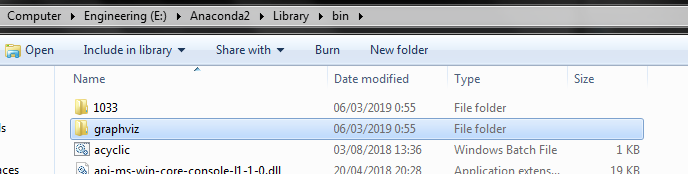
\includegraphics[scale=0.5]{figures/solusi3.png}
\caption{Folder Graphviz}
\label{Eror}
\end{figure}
\item
Salin alamat tersebut, kemudian buka Environment Variable dan Edit. 
\item
Pada bagian PATH pilih edit, dan salin alamat tersebut seperti berikut :
\begin{figure}[ht]
\centering
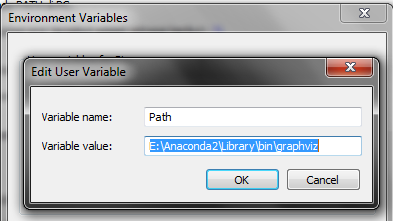
\includegraphics[scale=0.5]{figures/solusi4.png}
\caption{Menambahkan Graphviz kePATH}
\label{Eror}
\end{figure}
\item
Klik ok, kemudian restart Spyder dan jalankan kembali Skrip, maka hasilnya akan seperti berikut dan eror berhasil diselesaikan
\begin{figure}[ht]
\centering
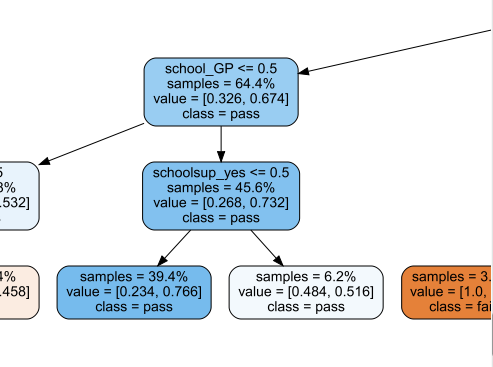
\includegraphics[scale=0.5]{figures/solusi5.png}
\caption{Evaluasi Eror}
\label{Eror}
\end{figure}
\end{itemize}
\end{enumerate}

\subsection{Error File Not Exist}
\begin{enumerate}
	\item
Berikut ini merupakan eror yang didapatkan saat menjalankan file csv sebagai dataset
\begin{figure}[ht]
\centering
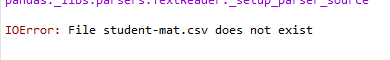
\includegraphics[scale=0.5]{figures/erorspyder2.png}
\caption{Error File Not Exist}
\label{Error}
\end{figure}
	\item
Pada gambar diatas kode erornya adalah IOError File student csv does not exist. Eror ini terjadi karena file yang dituju tidak berada didalam file yang salam dengan skrip ataupun filenya belum didefinisikan.
	\item
Solusi yang bisa dilakukan untuk mengatasi eror tersebut adalah sebagai berikut : \\
\begin{itemize}
\item
Buka Spyder, kemudian pada pojok kanan atas ada kolom sebagai berikut
\begin{figure}[ht]
\centering
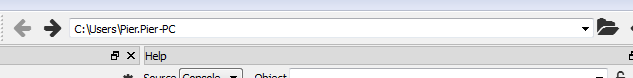
\includegraphics[scale=0.5]{figures/solusi6.png}
\caption{Kolom Direktori}
\label{Eror}
\end{figure}
\item
Pada kolom tersebut buka folder dimana file csv atau datasetnya tersimpan. Pada tutorial ini alamat foldernya sebagai berikut
\begin{figure}[ht]
\centering

\includegraphics[scale=0.5]{figures/solusi7.png}
\caption{Memasuki Direktori Dataset}
\label{Eror}
\end{figure}
\item
Kemudian jalankan lagi skrip tadi, akan berhasil seperti dibawah ini dan eror terselesaikan
\begin{figure}[ht]
\centering
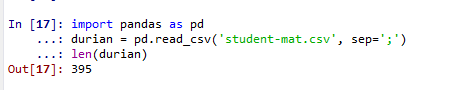
\includegraphics[scale=0.5]{figures/solusi8.png}
\caption{Evaluasi Error}
\label{Eror}
\end{figure}
\end{itemize}
\end{enumerate}

\section{Annisa Fathoroni/1164067}
\subsection{Teori}
Penyelesaian Tugas Harian 3 ( No. 1-7 )
\begin{enumerate}
\item Binary Classification Dan Ilustrasi Gambarnya
\begin{itemize}
\item Pengertian Binary Classification / Klasifikasi Biner:

Klasifikasi biner atau binomial adalah tugas untuk mengklasifikasikan elemen-elemen dari himpunan tertentu ke dalam dua kelompok (memprediksi kelompok mana yang masing-masing dimiliki) berdasarkan aturan klasifikasi. Klasifikasi biner adalah dikotomisasi yang diterapkan untuk tujuan praktis, dan dalam banyak masalah klasifikasi biner praktis, kedua kelompok tidak simetris - daripada akurasi keseluruhan, proporsi relatif dari berbagai jenis kesalahan yang menarik. Misalnya, dalam pengujian medis, false positive (mendeteksi penyakit ketika tidak ada) dianggap berbeda dari false negative (tidak mendeteksi penyakit ketika hadir).

\item Ilustrasi Gambar Binary Classification:

\begin{figure}[ht]
\centering
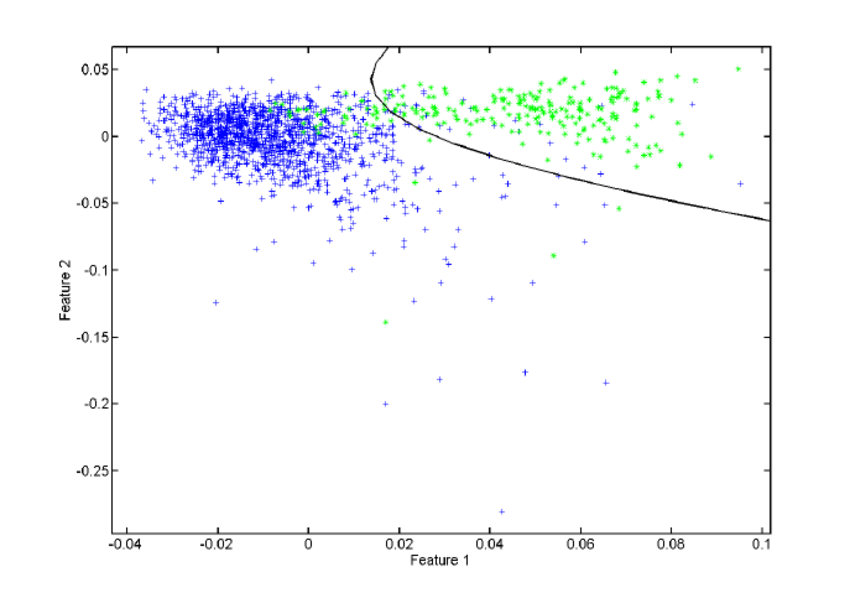
\includegraphics[scale=0.5]{figures/Chapter2-AnnisaFathoroni1.png}
\caption{capturing}
\label{contoh}
\end{figure}
\end{itemize}

\item Supervised Learning, Unsupervised Learning, Clustering Dan Ilustrasi Gambar
\begin{itemize}
\item Pengertian Supervised Learning dan Unsupervised Learning:

Supervised learning adalah sebuah pendekatan dimana sudah terdapat data yang dilatih, dan terdapat variable yang ditargetkan sehingga tujuan dari pendekatan ini adalah mengkelompokan suatu data ke data yang sudah ada, lain halnya dengan unsupervised learning, unsupervised learning tidak memiliki data latih, sehingga dari data yang ada, kita mengelompokan data tersebut menjadi 2 bagian atau 3 bagian dan seterusnya.

\begin{itemize}
\item Ilustrasi Gambar Supervised Learning dan Unsupervised Learning:

\begin{figure}[ht]
\centering
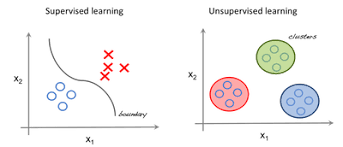
\includegraphics[scale=0.5]{figures/Chapter2-AnnisaFathoroni2.png}
\caption{capturing}
\label{contoh}
\end{figure}

\item Pengertian Clustering:

Clustering atau klasterisasi adalah metode pengelompokan data. Menurut Tan, 2006 clustering adalah sebuah proses untuk mengelompokan data ke dalam beberapa cluster atau kelompok sehingga data dalam satu cluster memiliki tingkat kemiripan yang maksimum dan data antar cluster memiliki kemiripan yang minimum. Clustering merupakan proses partisi satu set objek data ke dalam himpunan bagian yang disebut dengan cluster. Objek yang di dalam cluster memiliki kemiripan karakteristik antar satu sama lainnya dan berbeda dengan cluster yang lain. Partisi tidak dilakukan secara manual melainkan dengan suatu algoritma clustering. Oleh karena itu, clustering sangat berguna dan bisa menemukan group atau kelompokyang tidak dikenal dalam data. Clustering banyak digunakan dalam berbagai aplikasi seperti misalnya pada business inteligence, pengenalan pola citra, web search, bidang ilmu biologi, dan untuk keamanan (security). Di dalam business inteligence, clustering bisa mengatur banyak customer ke dalam banyaknya kelompok. Contohnya mengelompokan customer ke dalam beberapa cluster dengan kesamaan karakteristik yang kuat. Clustering juga dikenal sebagai data segmentasi karena clustering mempartisi banyak data set ke dalam banyak group berdasarkan kesamaannya. Selain itu clustering juga bisa sebagai outlier detection.

\begin{figure}[ht]
\centering
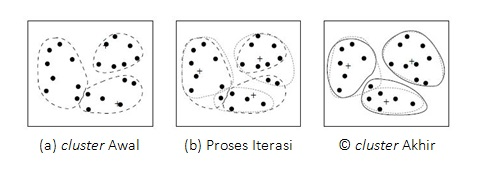
\includegraphics[scale=0.5]{figures/Chapter2-AnnisaFathoroni3.jpg}
\caption{capturing}
\label{contoh}
\end{figure}
\end{itemize}

\item Evaluasi, Akurasi Dan Ilustrasi Gambar

Evaluasi digunakan untuk memeriksa/memastikan dan mengevaluasi model dalam bekerja ( seberapa baik ) dengan mengukur keakuratannya. Kita juga dapat menanalisis kesalahan yang dibuat pada model yang dijalankan, tingkat kebingungan dan menggunakan matriks kebingunan. Accuracy akan didefinisikan sebagai presentasi kasus yang diklasifikasikan dengan benar. Accuracy lebih jelasnya adalah perbandingan kasus yang diidentifikasi benar dengan jumlah semua kasus.

\begin{figure}[ht]
\centering
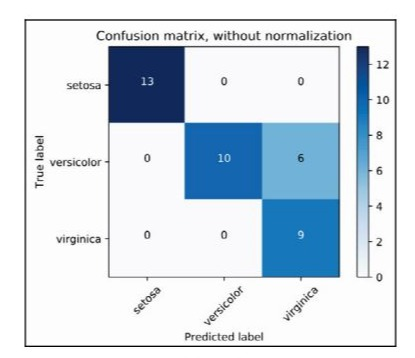
\includegraphics[scale=0.5]{figures/Chapter2-AnnisaFathoroni9.jpeg}
\caption{capturing}
\label{contoh}
\end{figure}

\begin{figure}[ht]
\centering
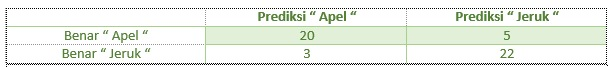
\includegraphics[scale=0.5]{figures/Chapter2-AnnisaFathoroni10.jpeg}
\caption{Akurasi}
\label{contoh}
\end{figure}

\item Cara membuat dan membaca confussion matrix:

Confusion matrix adalah suatu metode yang biasanya digunakan untuk melakukan perhitungan akurasi pada konsep data mining. Rumus ini melakukan perhitungan dengan 4 keluaran, yaitu: recall, precision, acuraccy dan error rate.
Rumus dari Error Rate = (b+c)/(a+b+c+d)
Keterangan:
jika hasil prediksi negatif dan data sebenarnya negatif.
jika hasil prediksi positif sedangkan nilai sebenarnya negatif.
jika hasil prediksi negatif sedangkan nilai sebenarnya positif.
jika hasil prediksi positif dan nilai sebenarnya positif.
Contoh perhitungan confusion matrix adalah sebagai berikut, yaitu pengambilan keputusan untuk mendapatkan bantuan beasiswa. Saya menggunakan dua atribut, yaitu rekening listrik dan gaji. Ini adalah pohon keputusannya:
yang pertama kita lakukan yaitu mencari 4 nilai yaitu a,b,c, dan d:
a= 5
b= 1
c= 1
d= 3
Kemudian kita dapat mencari nilai Recall, Precision, accuracy dan Error Rate:
Recall =3/(1+3) = 0,75
Precision = 3/(1+3) = 0,75
Accuracy =(5+3)/(5+1+1+3) = 0,8
Error Rate =(1+1)/(5+1+1+3) = 0,2

\begin{figure}[ht]
\centering
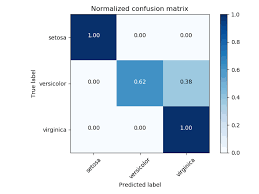
\includegraphics[scale=0.5]{figures/Chapter2-AnnisaFathoroni4.png}
\caption{capturing}
\label{contoh}
\end{figure}

\item Cara Bekerja K-Fold Cross Validation:

Total instance dibagi menjadi N bagian. 
Fold ke-1 adalah ketika bagian ke-1 menjadi data uji (testing data) dan 
Sisanya menjadi data latih (training data). Selanjutnya, hitung akurasi berdasarkan porsi data tersebut. Perhitungan akurasi tersebut dengan menggunakan persamaan sebagai berikut: 
Fold ke-2 adalah ketika bagian ke-2 menjadi data uji (testing data) dan sisanya menjadi data latih (training data). Selanjutnya, hitung akurasi berdasarkan porsi data tersebut.  
Demikian seterusnya hingga mencapai fold ke-K. Hitung rata-rata akurasi dari K buah akurasi di atas. Rata-rata akurasi ini menjadi akurasi final.

\begin{figure}[ht]
\centering
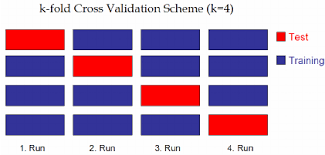
\includegraphics[scale=0.5]{figures/Chapter2-AnnisaFathoroni5.png}
\caption{capturing}
\label{contoh}
\end{figure}

\item Decision Tree

Decision tree adalah salah satu metode klasifikasi yang paling populer karena mudah diinterpretasikan oleh manusia. Decision tree digunakan untuk pengenalan pola dan termasuk dalam pengenalan pola secara statistik.

\begin{figure}[ht]
\centering
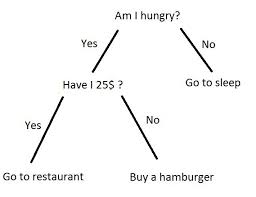
\includegraphics[scale=0.5]{figures/Chapter2-AnnisaFathoroni6.jpg}
\caption{capturing}
\label{contoh}
\end{figure}

\item Information Gain dan Entropi

Information gain adalah salah satu atribute selection measure yang digunakan untuk memilih test atribute tiap node pada tree. Atribut dengan information gain tertinggi dipilih sebagai test atribut dari suatu node. Ada 2 kasus berbeda pada saat penghitungan Information Gain, pertama untuk kasus penghitungan atribut tanpa missing value dan kedua, penghitungan atribut dengan missing value.

\begin{figure}[ht]
\centering
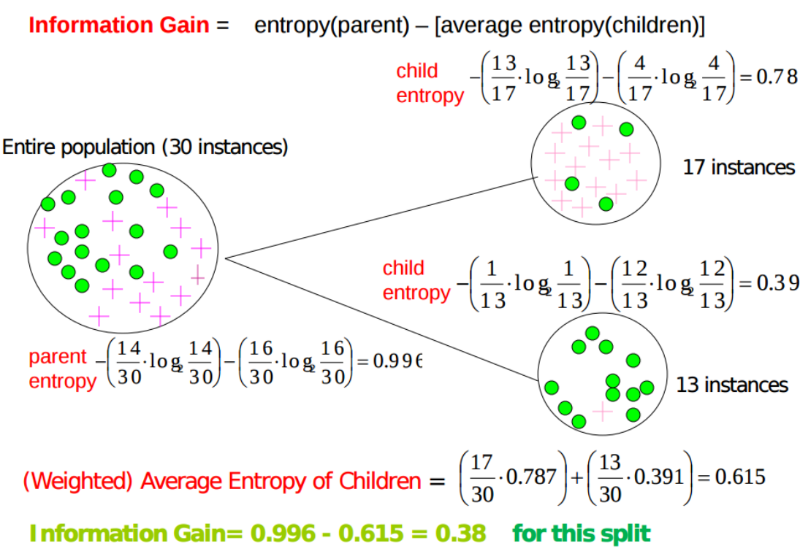
\includegraphics[scale=0.5]{figures/Chapter2-AnnisaFathoroni7.png}
\caption{capturing}
\label{contoh}
\end{figure}

Entropi adalah suatu parameter untuk mengukur tingkat keberagaman (heterogenitas) dari kumpulan data. Semakin heterogen, nilai entropi semakin besar. 
\begin{figure}[ht]
\centering
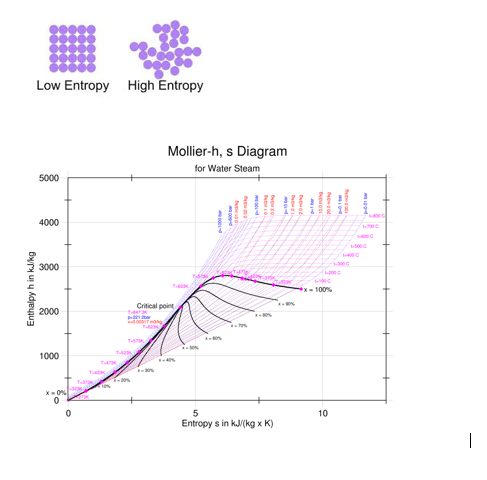
\includegraphics[scale=0.5]{figures/Chapter2-AnnisaFathoroni8.png}
\caption{capturing}
\label{contoh}
\end{figure}

\end{itemize}
\end{enumerate}

\section{Annisa Fathoroni/1164067}
\subsection{Praktek scikit-learn}
Penyelesaian Tugas Harian 4 ( No. 1-12 )
\begin{itemize}
\item Pembahasan Code dan Hasil.
\begin{enumerate}
\item Code 1.

Penjelasan: 

Pada code pertama menjelaskan membaca berapa banyak jumlah file yang terdapat pada file 'student-por.csv'.

\begin{itemize}

\item Hasil Code 1:
\begin{figure}[ht]
\centering
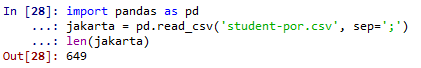
\includegraphics[scale=0.4]{figures/AnnisaFathoroni-1.png}
\caption{Hasil Code 1}
\label{contoh}
\end{figure}

\end{itemize}

\item Code 2.

Penjelasan:

Pada code kedua menjelaskan variabel jakarta akan menampilkan baris G1, G2 dan G3 dengan ketentuan lebih dari 35 maka akan muncul secara live atau langsung data yang diperintahkan pada code tersebut.

\begin{itemize}


\item Hasil Code 2:

\begin{figure}[ht]
\centering
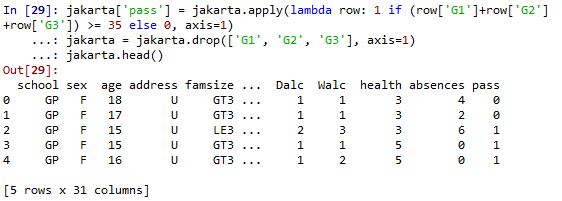
\includegraphics[scale=0.4]{figures/AnnisaFathoroni-2.png}
\caption{Hasil Code 2}
\label{contoh}
\end{figure}

\end{itemize}

\item Code 3.

Penjelasan:

Pada code ketiga menjelaskan variabel jakarta memanggil fungsi dummies yang memiliki beberapa kolom yang akan ditampilkan apabila perintah print dilakukan.
 
\begin{itemize}


\item Hasil Code 3:

\begin{figure}[ht]
\centering
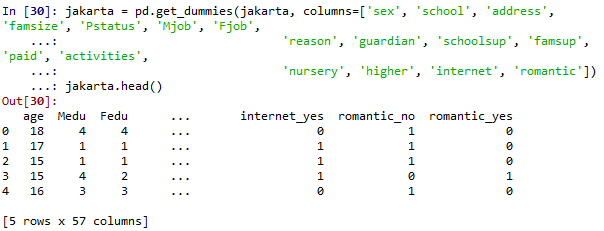
\includegraphics[scale=0.4]{figures/AnnisaFathoroni-3.png}
\caption{Hasil Code 3}
\label{contoh}
\end{figure}

\end{itemize}


\item Code 4.
\par Penjelasan:
\par 
Pada code keempat variabel solok akan menampilkan sampel data dari 500 training data dan 500 tetsing data. Kemudian data akan dicetak atau di print dari training data dan testing data.
\begin{itemize}
\par
\item Hasil Code 4:

\begin{figure}[ht]
\centering
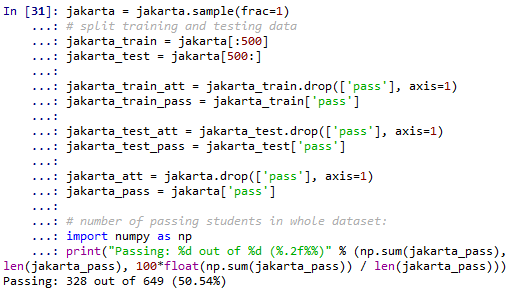
\includegraphics[scale=0.4]{figures/AnnisaFathoroni-4.png}
\caption{Hasil Code 4}
\label{contoh}
\end{figure}

\end{itemize}
\par
\item Code 5.
\par Penjelasan:
\par 
Pada code kelima menguji klasifikasi Decision Tree apakah berjalan dengan yang sudah ditentukan atau tidak.
\begin{itemize}
\par
\item Hasil Code 5:

\begin{figure}[ht]
\centering
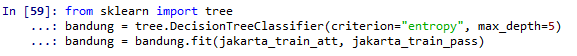
\includegraphics[scale=0.4]{figures/AnnisaFathoroni-5.png}
\caption{Hasil Code 5}
\label{contoh}
\end{figure}

\end{itemize}
\par
\item Code 6.
\par Penjelasan:
\par 
Pada code keenam menampilkan decision tree.
\begin{itemize}
\par
\item Hasil Code 6:

\begin{figure}[ht]
\centering
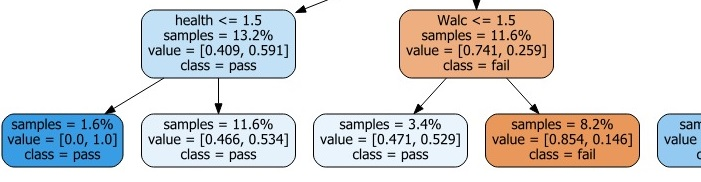
\includegraphics[scale=0.4]{figures/AnnisaFathoroni-6a.jpeg}
\caption{Hasil Code 6}
\label{contoh}
\end{figure}

\end{itemize}
\par
\item Code 7.
\par Penjelasan:
\par 
Pada code ketujuh akan menampilkan yang terdapat pada Library Graphviz, apabila benar akan menampilkan hasil output seperti yang terdapat pada gambar atau kalau pengujian gagal akan terdapat error.
\begin{itemize}
\par
\item Hasil Code 7:

\begin{figure}[ht]
\centering
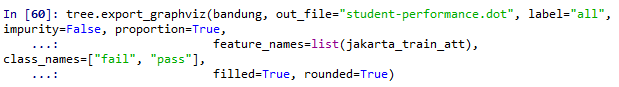
\includegraphics[scale=0.4]{figures/AnnisaFathoroni-7.png}
\caption{Hasil Code 7}
\label{contoh}
\end{figure}

\end{itemize}
\par
\item Code 8.
\par Penjelasan:
\par 
Pada code kedelapan menampilkan hasil perhitungan dari kedua parameter yang terdapat pada code tersebut.
\begin{itemize}
\par
\item Hasil Code 8:

\begin{figure}[ht]
\centering
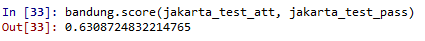
\includegraphics[scale=0.4]{figures/AnnisaFathoroni-8.png}
\caption{Hasil Code 8}
\label{contoh}
\end{figure}

\end{itemize}
\par
\item Code 9.
\par Penjelasan:
\par 
Pada code kesembilan membaca isi dari library, memanggil score yang terdapat pada parameter code tersebut. Sehingga apabila di print memanggil hasil output akan menghasilkan sebuah angka akurasi.
\begin{itemize}
\par
\item Hasil Code 9:

\begin{figure}[ht]
\centering
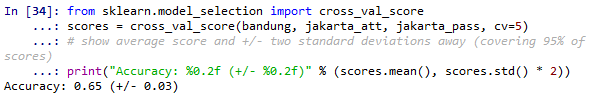
\includegraphics[scale=0.4]{figures/AnnisaFathoroni-9.png}
\caption{Hasil Code 9}
\label{contoh}
\end{figure}

\end{itemize}
\par
\item Code 10.
\par Penjelasan:
\par
Pada code kesepuluh menampilkan hasil dari fungsi Max Depth dan Accuraccy dari dari Decission Tree. Yaitu menmpilkan data dari angka 1-20.
\begin{itemize}
\par
\item Hasil Code 10:

\begin{figure}[ht]
\centering
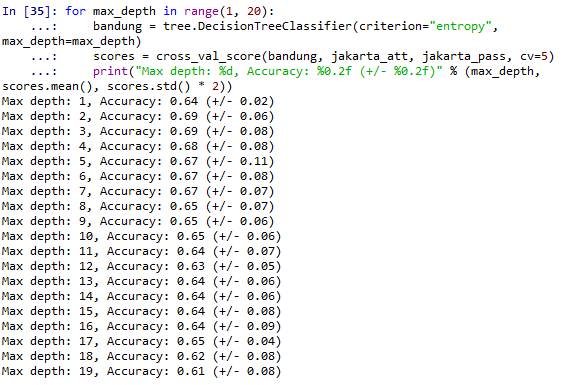
\includegraphics[scale=0.4]{figures/AnnisaFathoroni-10.png}
\caption{Hasil Code 10}
\label{contoh}
\end{figure}

\end{itemize}
\par
\item Code 11.
\par Penjelasan:
\par 
Pada code kesebelas menjelaskan variable scores akan menampilkan atau mendefinisikan nilai dari variabel score.
\begin{itemize}
\par
\item Hasil Code 11:

\begin{figure}[ht]
\centering
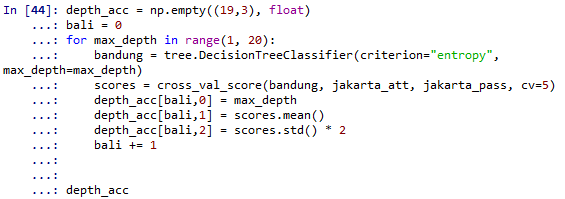
\includegraphics[scale=0.8]{figures/AnnisaFathoroni-11a.png}
\caption{Hasil Code 11}
\label{contoh}
\end{figure}

\begin{figure}[ht]
\centering
\includegraphics[scale=0.8]{figures/AnnisaFathoroni-11b.png}
\caption{Hasil Code 11}
\label{contoh}
\end{figure}

\end{itemize}
\par
\item Code 12.
\par Penjelasan:
\par 
Pada code kedua belas menjelaskan pada library matplotlib akan menampilkan gambar grafik pada gambar 12 dari eksekusi fungsi ax.errorbar.
\begin{itemize}
\par
\item Hasil Code 12:

\begin{figure}[ht]
\centering
\includegraphics[scale=0.6]{figures/AnnisaFathoroni-12.png}
\caption{Hasil Code 12}
\label{contoh}
\end{figure}

\end{itemize}
\end{enumerate}

\subsection{Praktek Penanganan Error}

\begin{figure}[ht]
\centering
\includegraphics[scale=0.4]{figures/AnnisaFathoroni-6.png}
\caption{HASIL YANG MASIH ERROR}
\label{contoh}
\end{figure}

\begin{verbatim}
Traceback (most recent call last):

  File "<ipython-input-33-b4843d06cfa2>", line 1, in <module>
    import graphviz

ModuleNotFoundError: No module named 'graphviz'
\end{verbatim}

Solusi dari error tersebut adalah memasukkan path dari graphviz ke environment variabels, maka akan menampilkan hasil yaitu sebuah decision tree.

\end{itemize}

\section{Annisacahyani/1164066}
\subsection{Teori}
Penyelesaian Tugas Harian 3 ( No. 1-7 )
\begin{enumerate}
\item Binary Classification Dan Ilustrasi Gambarnya
\begin{itemize}
\item Pengertian Binary Classification / Klasifikasi Biner:
\par Klasifikasi biner atau binomial adalah tugas untuk mengklasifikasikan elemen-elemen dari himpunan tertentu ke dalam dua kelompok (memprediksi kelompok mana yang masing-masing dimiliki) berdasarkan aturan klasifikasi.
\end{itemize}
\end{enumerate}

\begin{enumerate}
\item Supervised Learning, Unsupervised Learning, Clustering Dan Ilustrasi Gambar
\begin{itemize}
\item Pengertian Supervised Learning, unsuvised learning,dan clustering :
\par Supervised learning adalah tugas pembelajaran mesin untuk mempelajari fungsi yang memetakan input ke output berdasarkan contoh pasangan input-output. Unsupervised learning yaitu istilah yang digunakan untuk pembelajaran bahasa Ibrani, yang terkait dengan pembelajaran tanpa guru, juga dikenal sebagai organisasi mandiri dan metode pemodelan kepadatan probabilitas input. Dan Clustering dapat dianggap sebagai masalah pembelajaran tanpa pengawasan yang paling penting jadi, karena setiap masalah lain dari jenis ini, ini berkaitan dengan menemukan struktur dalam kumpulan data yang tidak berlabel.
\end{itemize}
\end{enumerate}

\begin{enumerate}
\item Evaluasi, Akurasi Dan Ilustrasi Gambar
\begin{itemize}
\item Pengertian Evaluasi
\par Evaluasi ini digunakan untuk memeriksa atau memastikan dan mengevaluasi model dalam bekerja ( seberapa baik ) dengan mengukur keakuratannya. Sehingga kita juga dapat menanalisis kesalahan yang dibuat pada model yang dijalankan, sehingga tingkat kebingungan yang menggunakan matriks kebingunan.
\end{itemize}
\end{enumerate}

\begin{enumerate}
\item Membuat Dan Membaca Confusion Matrix Beserta Contoh
\end{enumerate}
\begin{itemize}
\item Pengertian Confusion Matrix
\par Confusion matrix adalah suatu metode yang biasanya digunakan untuk melakukan sebuah perhitungan akurasi pada konsep data mining atau Sistem Pendukung Keputusan. Pada pengukuran kinerja menggunakan confusion matrix, terdapat 4 (empat) istilah sebagai representasi hasil proses klasifikasi. Keempat istilah tersebut adalah True Positive (TP), True Negative (TN), False Positive (FP) dan False Negative(FN).
\par
\item Pembacaan Confusion Matrix
\begin{enumerate}
\item Jika hasil prediksi menghasilkan negatif dan data yang sebenarnya itu merupakan negatif.
\item Jika hasil prediksi menghasilkan positif sedangkan nilai yang sebenarnya itu merupakan negatif.
\item Jika hasil prediksi menghasilkan negatif sedangkan nilaiyang sebenarnya itu merupakan positif.
\item Jika hasil prediksi menghasilkan yang positif dan nilai sebenarnya merupakan positif.
\end{enumerate}
\par
\par
\item Pembuatan Confusion Matrix
\begin{enumerate}
\item Yang pertama yaitu untuk menentukan 4 proses klasifikasi yang akan kita gunakan dalam confusion matrix.
\item Kemudian 4 Istilah yang ada tersebut yaitu ada True Positive ( TP ), True Negative ( TN ), False Positive ( FP ) dan False Negative ( FN ).
\item Kemudian kita kelompokkan klasifikasi tersebut dengan menggunakan klasifikasi biner
\item Kemudian dari hal tersebut akan menghasilkan keluaran berupa 2 Kelas yaitu ( Positif dan Negatif ) dan penentuan TP, FP ( 1 klasifikasi positif ) , FN dan TN ( 1 klasifikasi negatif ).
\end{enumerate}
\par
\end{itemize}

\par
\begin{itemize}
\item Penjelasan
\begin{enumerate}
\item Recall
\par Dari semua kelas positif, seberapa banyak yang kami prediksi dengan benar. Itu harus setinggi mungkin.
\par

\par
\end{enumerate}
\end{itemize}

\begin{itemize}
\item Cara Kerja K-Fold Classification Dan Ilustrasi Gambar
\begin{enumerate}
\item Pertama kita total instance dibagi menjadi N bagian.
\item Kemudian Fold ke-1 adalah ketika bagian ke-1 menjadi data uji (testing data) dan sisanya menjadi data latih (training data).
\item Setelah itu fold yang ke-2 adalah ketika bagian ke-2 menjadi data uji (testing data) dan sisanya menjadi data latih (training data). 
\item Demikian sampai seterusnya hingga mencapai fold ke-K. Hitung rata-rata akurasi dari K buah akurasi di atas.Rata-rata akurasi ini menjadi akurasi final
\end{enumerate}
\end{itemize}

\begin{enumerate}
\item Decision Tree Dan Ilustrasi Gambar
\begin{itemize}
\item Pengertian Decision Tree
\par Decision Tree yaitu alat pendukung keputusan yang menggunakan model keputusan seperti pohon dan konsekuensinya yang mungkin, termasuk hasil acara kebetulan, biaya sumber daya, dan utilitas.
\end{itemize}
\end{enumerate}

\par

\begin{enumerate}
\item Information Gain Dan Entropi
\begin{itemize}
\item Pengertian Information Gain dan entropi
\par information gain didasarkan pada penurunan entropi setelah dataset dibagi pada atribut. Membangun pohon keputusan adalah semua tentang menemukan atribut yang mengembalikan perolehan informasi tertinggi. Sedangkan Entropi itu dibangun dari atas ke bawah dari simpul akar dan melibatkan mempartisi data ke dalam himpunan bagian yang berisi instance dengan nilai yang sama yaitu homogen. 
\end{itemize}
\end{enumerate}


\section{Annisa Cahyani/1164066}
\subsection{Praktek Scikit-Learn}
Penyelesaian Tugas Harian 4 ( No. 1-12 )
\begin{enumerate}
\item Pembahasan Codingan Dan Hasilnya
\begin{enumerate}
\item Codingan Pertama :
\par Penjelasan : Codingan pertama ini akan meload ( menampilkan ) data pada file yang ditentukan. Untuk codingan ini file yang dieksekusi ialah " student-mat.csv " . 
\par
\begin{itemize}
\par
\item Hasil Codingan Pertama :
\par

\begin{figure}[ht]
\centering
\includegraphics[scale=0.6]{figures/hasil1.jpg}
\caption{codingan pertama}
\label{contoh}
\end{figure}

\par
\end{itemize}
\item Codingan Kedua :
\par Penjelasan : Codingan kedua ini secara keseluruhan yaitu akan menampilkan  baris  G1, G2 dan G3 ( berdasarkan kriterianya ) untuk kolom PASS pada variabel.
\par 
\begin{itemize}
\par
\item Hasil Codingan Kedua :

\begin{figure}[ht]
\centering
\includegraphics[scale=0.6]{figures/hasil2.jpg}
\caption{codingan kedua}
\label{contoh}
\end{figure}

\end{itemize}
\par
\item Codingan Ketiga :
\par Penjelasan : Secara keseluruhan, codingan ini akan  mendefinisikan pemanggilan ke get dummies dari pizza dalam variabel bakso. Di dalam get dummies sendiri akan terdefinisikan variabel  dengan kolom-kolom yang akan dieksekusi seperti school, address dll
\par 
\begin{itemize}
\par
\item Hasil Codingan Ketiga :

\begin{figure}[ht]
\centering
\includegraphics[scale=0.4]{figures/hasil3.jpg}
\caption{codingan ketiga}
\label{contoh}
\end{figure}

\end{itemize}
\par
\item Codingan Keempat :
\par Penjelasan : Secara keseluruhan codingan ini difungsikan untuk mendefinisikan pembagian data yang berupa training dan testing data. Secara jelasnya pertama-tama variabel  akan mendefinisikan sampel yang akan digunakan ( berupa shuffle row ) . Nah kemudian masing-masing dari  parameter tersebut akan berjumlah 500 data ( telah dibagi untuk training dan testing ).
\par 
\begin{itemize}
\par
\item Hasil Codingan Keempat :

\begin{figure}[ht]
\centering
\includegraphics[scale=0.4]{figures/hasil4.jpg}
\caption{codingan keempat}
\label{contoh}
\end{figure}

\end{itemize}
\par
\item Codingan Kelima :
\par Penjelasan : Secara keseluruhan, codingan ini hanya membuktikan pada bagian pengujian dari Klasifikasi Decision Tree yang ada, apakah true atau tidak dan hasilnya true. Apabila dibahas dengan  lengkap maka pada codingan ini di definisikan library sklearn untuk mengimpor atau menampilkan tree.
\par 
\begin{itemize}
\par
\item Hasil Codingan Kelima :

\begin{figure}[ht]
\centering
\includegraphics[scale=0.4]{figures/hasil5.jpg}
\caption{codingan kelima}
\label{contoh}
\end{figure}

\end{itemize}
\par
\item Codingan Keenam :
\par Penjelasan : Codingan ini memberikan gambaran dari klasifikasi decision tree dari pengolahan parameter tersebut ada yang dieksekusi kedalam variabel. Tentunya dengan pemanfaatan library graphviz yang telah diimport dan difungsikan.
\par 
\begin{itemize}
\par
\item Hasil Codingan Keenam :

\begin{figure}[ht]
\centering
\includegraphics[scale=0.4]{figures/hasil6.jpg}
\caption{supervised}
\label{contoh}
\end{figure}

\end{itemize}
\par
\item Codingan Ketujuh :
\par Penjelasan : Secara keseluruhan, codingan ini membahas tentang penyimpanan tree dari library graphiz yang dieksekusi bersamaan dengan variabel dan parameter lainnya. Dilakukan pengecekan dan pengujian apakah klasifikasi decision treenya dapat berjalan atau tidak
\par 
\begin{itemize}
\par
\item Hasil Codingan Ketujuh :

\begin{figure}[ht]
\centering
\includegraphics[scale=0.4]{figures/hasil7.jpg}
\caption{codingan ketujuh}
\label{contoh}
\end{figure}

\end{itemize}
\par
\item Codingan Kedelapan :
\par Penjelasan : Secara keseluruhan, codingan ini membaca score dari variabel sate dimana terdapat 2 parameter yang dihitung dan diuji. Untuk hasilnya sendiri mengapa hasilnya berupa angka, dikarenakan pada parameter yang dieksekusi memang memiliki data sehingga dieksekusi dan menghasilkan keluaran dari score tersebut.
\par 
\begin{itemize}
\par
\item Hasil Codingan Kedelapan :

\begin{figure}[ht]
\centering
\includegraphics[scale=0.4]{figures/hasil8.jpg}
\caption{codingan kedelapan}
\label{contoh}
\end{figure}

\end{itemize}
\par
\item Codingan Kesembilan :
\par Penjelasan : Secara keseluruhan, codingan ini membahas tentang pengkesekusian fungsi dan variabel dari library yang didefinisikan dan yang diimport. Penjelasan lebih jelasnya ialah codingan ini mendefinisikan library sklearn.model.selection kemudian mengimpor cross val score. Kemudian variabel score mendefinisikan cross val score yang telah diimport tadi dengan 4 parameter.
\par 
\begin{itemize}
\par
\item Hasil Codingan Kesembilan :

\begin{figure}[ht]
\centering
\includegraphics[scale=0.7]{figures/hasil9.jpg}
\caption{codingan kesembilan}
\label{contoh}
\end{figure}

\end{itemize}
\par
\item Codingan Ke-10 :
\par Penjelasan : Codingan ini mendefinisikan max depth dalam jarak angka antara parameter yang ke 1 dan 20. Variabel  mendefinisikan klasifier decision tree dengan 2 parameter.
\par 
\begin{itemize}
\par
\item Hasil Codingan Ke-10 :

\begin{figure}[ht]
\centering
\includegraphics[scale=0.6]{figures/hasil10.jpg}
\caption{codingan ke-10}
\label{contoh}
\end{figure}

\end{itemize}
\par
\item Codingan Ke-11 :
\par Penjelasan : Codingan ini mendefinisikan bahwa variabel cahya akan mengeksekusi empty dari importan library numphy yang dinamakan np dengan 2 parameter yaitu 19,3 dan float. i didefinisikan dengan angka 0 kemudian untuk perhitungan jarak max depth diantara parameter 1 dan 20. Variabel yang  mendefinisikan klasifikasi decision tree dengan 2 parameter. 
\par 
\begin{itemize}
\par
\item Hasil Codingan Ke-11 :

\begin{figure}[ht]
\centering
\includegraphics[scale=0.3]{figures/hasil11.jpg}
\caption{codingan ke-11}
\label{contoh}
\end{figure}

\end{itemize}
\par
\item Codingan Ke-12 :
\par Penjelasan : Codingan ini mendefinisikan untuk pemanggilan dari library matplotlib.pyplot sebagai cahya sehingga nanti hasilnya akan berbentuk gambar grafik/gelombang.
\par 
\begin{itemize}
\par
\item Hasil Codingan Ke-12 :

\begin{figure}[ht]
\centering
\includegraphics[scale=0.4]{figures/hasil12.jpg}
\caption{supervised}
\label{contoh}
\end{figure}

\end{itemize}
\end{enumerate}
\end{enumerate}

\subsection{Penanganan Error}
\par Pembahasan dan Penyelesaiian Error
\par
\begin{enumerate}
\item Error 1	: 
\par
\par

\begin{figure}[ht]
\centering
\includegraphics[scale=0.4]{figures/errorr.jpg}
\caption{error 1}
\label{contoh}
\end{figure}

\par
\begin{itemize}
\item Penjelasan	: 
\begin{itemize}
\item Pada error tersebut  dapat dikatakan bahwa untuk file -b"student-mat.csv" tidak ada. Mengapa? karena file pada codingan yang dieksekusi yaitu student-performance.py tidak berada pada folder yang sama.
\item Silahkan menambahkan fungsi yang mendefinisikan folder tempat file "student-mat.csv berada. 
\item Silahkan tambahkan perintah " dataset/student-mat.csv " pada codingannya
\item Dengan penambahan perintah tersebut maka tidak akan terjadi error lagi.
\end{itemize}
\end{itemize}

\end{enumerate}